\section[Weryfikacja]{Część weryfikacyjna}\label{sec:verification} % 30-40% - opis wyników, analiza, weryfikacja i porównanie do danych literaturowych
    Niniejsza analiza przeprowadzona została na ``finalnej'' w chwili pisania
    niniejszej pracy wersji programu.  W repozytorium Git na GitHubie jest to
    commit ``placeholder'' \todo[inline]{uzupełnić commita} identyfikowany
    również jako wersja 1.0.

    \subsection{Przypadki testowe}

    Kod przetestowano w dwojaki sposób. Pierwszym z nich są testy jednostkowe.
    Automatyczne testy jednostkowe uruchamiane po każdej wymiernej zmianie kodu
    pozwalają kontrolować działanie programu znacznie ułatwiają zapobieganie
    błędom.

    Poszczególne algorytmy podlegały testom przy użyciu ogólnodostępnego
    pakietu \code{pytest} i w większości były
    uruchamiane na platformie TravisCI\@.

    \subsubsection{Testy algorytmiczne}
    Testy algorytmiczne polegały na przeprowadzeniu fragmentu symulacji --- w
    przypadku testów algorytmów było to na przykład wygenerowanie pojedynczej
    cząstki o jednostkowej prędkości oraz zdepozytowanie jej gęstości prądu na
    siatkę, co pozwala porównać otrzymany wynik z przewidywanym analitycznie
    dla danego rozmiaru siatki i położenia cząstki.
    \begin{enumerate}
        \itemi{} \english{Gather} --- \code{test\_current\_deposition}, \code{test\_charge\_deposition}
            \begin{enumerate}
                \itemii{} Depozycja prądu lub ładunku z pojedynczej cząstki na niewielką siatkę i porównanie z wynikiem analitycznym\cite{Jablonski-notes}
                \itemii{} Depozycja prądu lub ładunku z dwóch pojedynczych cząstek na niewielką
                    siatkę i porównanie z sumą prądów lub ładunków dla obu pojedynczyczh
                    cząstek
                \itemii{} Depozycja prądu z dużej ilości równomiernie rozłożonych
                    cząstek --- weryfikacja średniej wartości prądu
                \itemii{} Depozycja prądu lub ładunku z cząstek blisko granic i porównanie z zamierzonymi warunkami brzegowymi
                \itemii{} Depozycja prądu dla cząstki poruszającej się powyżej prędkości światła --- procedura depozycji zwraca błąd
            \end{enumerate}

        \itemi{} \english{Solve} --- \code{test\_FieldSolver}, \code{test\_LongitudinalSolver}
            \begin{enumerate}
                \itemii{} Test \english{solvera} spektralnego poprzez
                    rozwiązanie równania Poissona dla sinusoidalnej, deltowej i rosnącej liniowo
                    dystrybucji ładunku. Weryfikacja dokładności rozwiązania i energii pola
                \itemii{} Test \english{solvera} rotacyjnego poprzez porównanie z rezultatami analitycznymi dla pojedynczych iteracji
            \end{enumerate}

        \itemi{} \english{Scatter} --- \code{test\_field\_interpolation} --- porównanie interpolowanego pola z przypadkiem analitycznym dla kilku prostych rozkładów pola

        \itemi{} \english{Push} --- \code{test\_pusher}
            \begin{enumerate}
                \itemii{} Ruch w jednorodnym polu elektrycznym wzdłuż osi układu,
                    w wersji nierelatywistycznej i relatywistycznej. Prędkość cząstki rośnie
                    jednostajnie w reżimie nierelatywistycznym.
                \itemii{} Relatywistyczny i nierelatywistyczny ruch kołowy z
                    zachowaniem energii w jednorodnym polu magnetycznym w kierunku osi $\hat{z}$. 
                \itemii{} Relatywistyczny ruch w potencjale oscylatora harmonicznego. Ruch cząstki jest porównany
                    z trajektorią obliczoną analitycznie w przypadku relatywistycznym.
                \itemii{} Zachowanie energii ruchu cząstki bez pola elektrycznego przy wysoce relatywistycznej prędkości, w kierunku ruchu oraz z prędkościami
                    w trzech wymiarach.
                \itemii{} Test dryfu $\vec{E} \times \vec{B}$ --- cząstka w skrzyżowanych polach elektrycznym i magnetycznym uzyskuje stabilną prędkość $E/B$.
                \itemii{} Test warunków brzegowych dla symulacji okresowych --- zachowanie liczby cząstek przechodzących przez granicę obszaru symulacji.
                \itemii{} Test warunków brzegowych dla symulacji okresowych --- spadek liczby cząstek przechodzących przez granicę obszaru symulacji do zera.
            \end{enumerate}
    \end{enumerate}

    \subsection{Testy symulacyjne --- przypadki elektrostatyczne}
    Testy symulacyjne polegały na uruchomieniu niewielkiej symulacji testowej z
    różnymi warunkami brzegowymi i ilościowym, automatycznym bądź jakościowym, wizualnym zweryfikowaniu
    dynamiki zjawisk w niej zachodzących.

    Zastosowano kod do symulacji kilku znanych problemów w fizyce plazmy:
    \subsubsection{oscylacje zimnej plazmy}
    Jest to efektywnie elektrostatyczna fala stojąca. Symulacja zaczyna z ujemnymi cząstkami
o zerowej prędkości początkowej, rozłożonymi w okresowym pudełku symulacyjnym
równomiernie z nałożonym na nie sinusoidalnym zaburzeniem:

\begin{align}
x &= x_0 + x_1\\
x_0 &= L * n / N\\
x_1 &= A  \sin(k x_0) = A \sin(2 \pi n x_0 / L)
\end{align}

Określenie ``zimna plazma'' bierze się z nietermalnego, deltowego
rozkładu prędkości cząstek --- jest to faktycznie strumień cząstek o stałej
(w tym szczególnym przypadku zerowej) prędkości.

Gęstość ładunku jest wyzerowana w pierwszym kroku algorytmu rozwiązywania pola elektrycznego
poprzez wyzerowanie zerowej składowej fourierowskiej gęstości ładunku, co jest jednoznaczne
z przyjęciem nieskończenie masywnych i nieruchomych jonów dodatnich dokładnie neutralizujących gęstość
ładunku elektronów.

Sytuacja ta
pozwala na obserwację oscylacji cząstek wokół ich stabilnych położeń
równowagi. W przestrzeni fazowej $x, V_x$ cząstki zataczają efektywnie
elipsy, co pozwala wnioskować że ruch ten jest z dobrym przybliżeniem harmoniczny.
Oczywiście, nie jest to do końca oscylacja harmoniczna z powodu odchyleń pola interpolowanego
z Eulerowskiej siatki od generowanego faktycznym potencjałem $ \sim x^2 $.

Jest to, oczywiście, spełnione jedynie dla niewielkich odchyleń; dla $A \to
dx$ obserwuje się nieliniowy reżim oscylacji, 

Symulacja ta jest wykorzystywana do weryfikacji podstawowych warunków, jakie powinna spełniać
symulacja elektrostatyczna --- na przykład długofalowe zachowanie energii, liczby cząstek (w układzie okresowym cząstki nie powinny
znikać).

\begin{figure}[h!]
  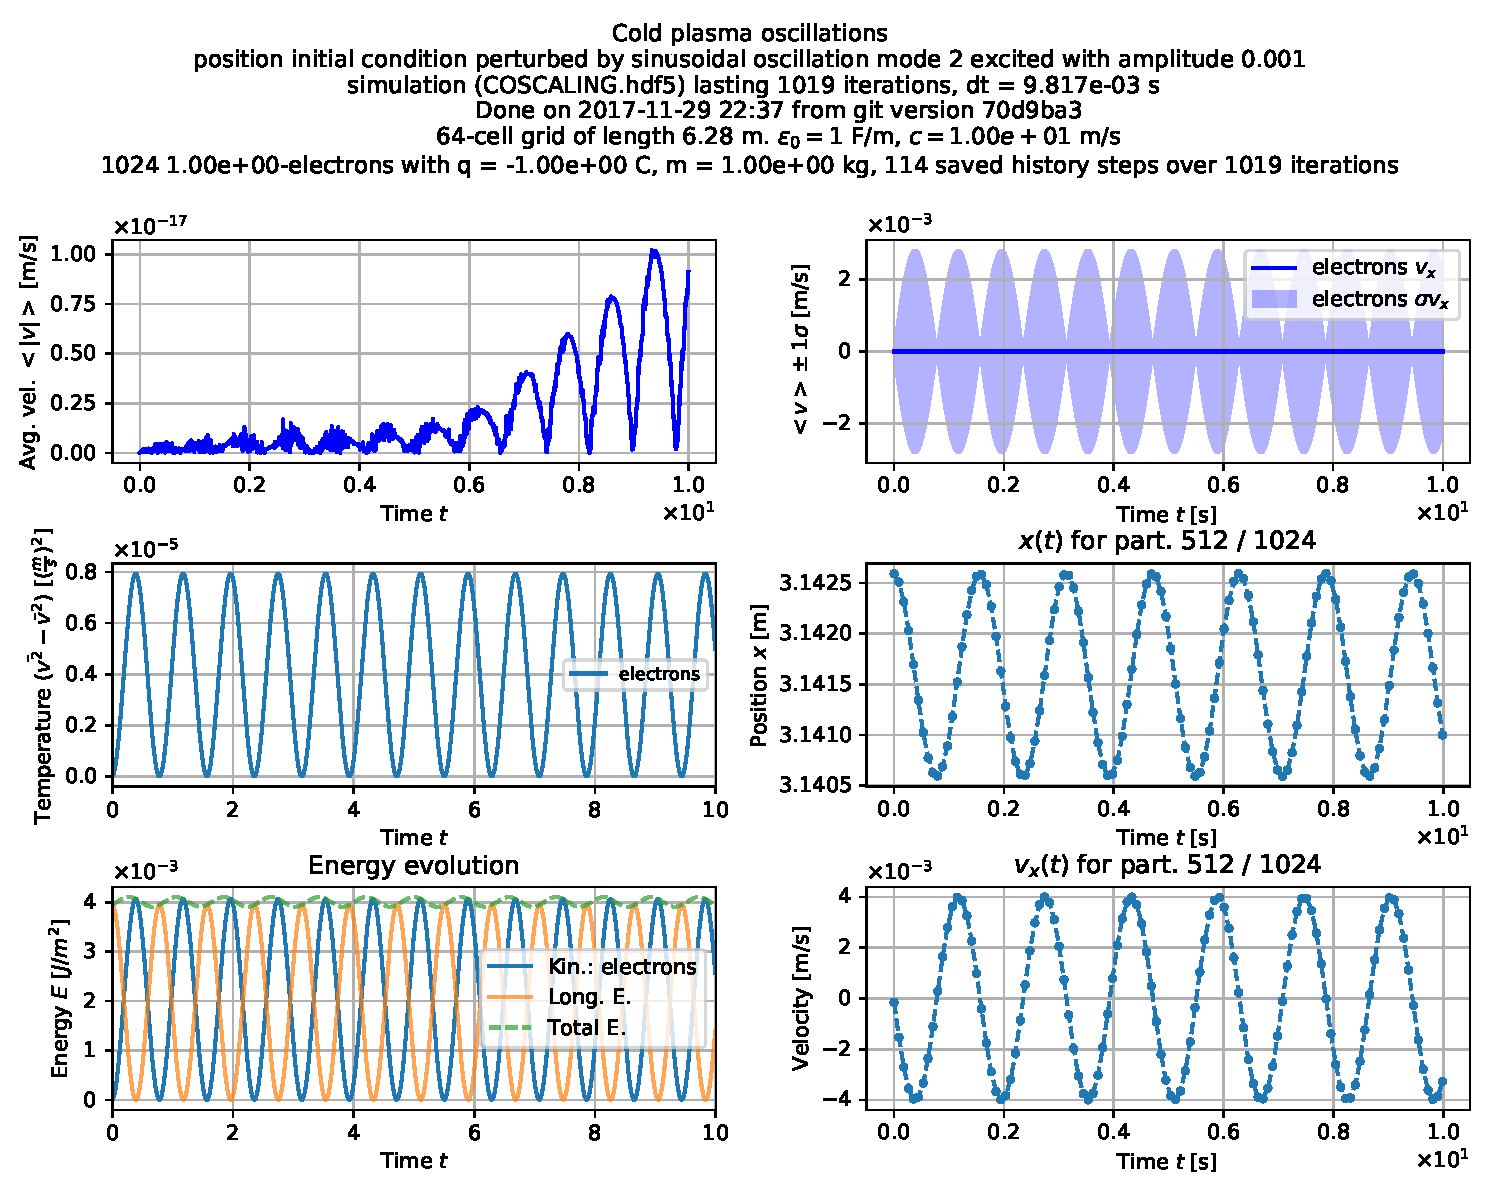
\includegraphics[width=\textwidth]{Images/COSCALING}
  \caption{Oscylacje zimnej plazmy w reżimie liniowym. Cząstki wykonują prawie harmoniczne oscylacje wokół swoich położeń równowagi, zaś energia
   w układzie jest wymieniana między energią kinetyczną cząstek a energią pola elektrostatycznego.\label{fig:coldplasma-linear}}
\end{figure}

Liniowy reżim obserwacji jest zaznaczony na rysunku~\ref{fig:coldplasma-linear}, zaś nieliniowy~\ref{fig:coldplasma-nonlinear}.

    \subsubsection{niestabilność dwóch strumieni}
W tym przypadku symulacja również zawiera zimną plazmę, lecz tym razem są to dwa strumienie ujemnych cząstek
o stałych, przeciwnych sobie prędkościach $v_0$ oraz $-v_0$.

    Dla niewielkich prędkości początkowych strumieni obserwuje się
    liniowy reżim oscylacji cząstek --- oba strumienie pozostają stabilne. Obserwuje się niewielkie oscylacje oraz
grupowanie się cząstek w rejony koherentnej większej gęstości wewnątrz strumienia (opisany przez Birdsalla i Langdona \emph{bunching}).

    Dla dużych prędkości obserwuje się nieliniowe
    zachowanie cząstek w przestrzeni fazowej. Oscylacje prędkości cząstek przybierają rząd wielkości porównywalny
    z początkową różnicą prędkości strumieni.
 Strumienie zaczynają się mieszać ze sobą nawzajem, zaś cały układ się termalizuje. Energia kinetyczna
 uporządkowanego ruchu strumieni zamienia się w energię potencjalną pola równowagowego 
oraz termalną energię kinetyczną, co sprawia, że średnia prędkość obu strumieni ulega zmniejszeniu. 

To oraz szybkość narastania niestabilności jest obiektem automatycznych testów sprawdzających poprawność symulacji.
% TODO TEST

\begin{figure}[h!]
  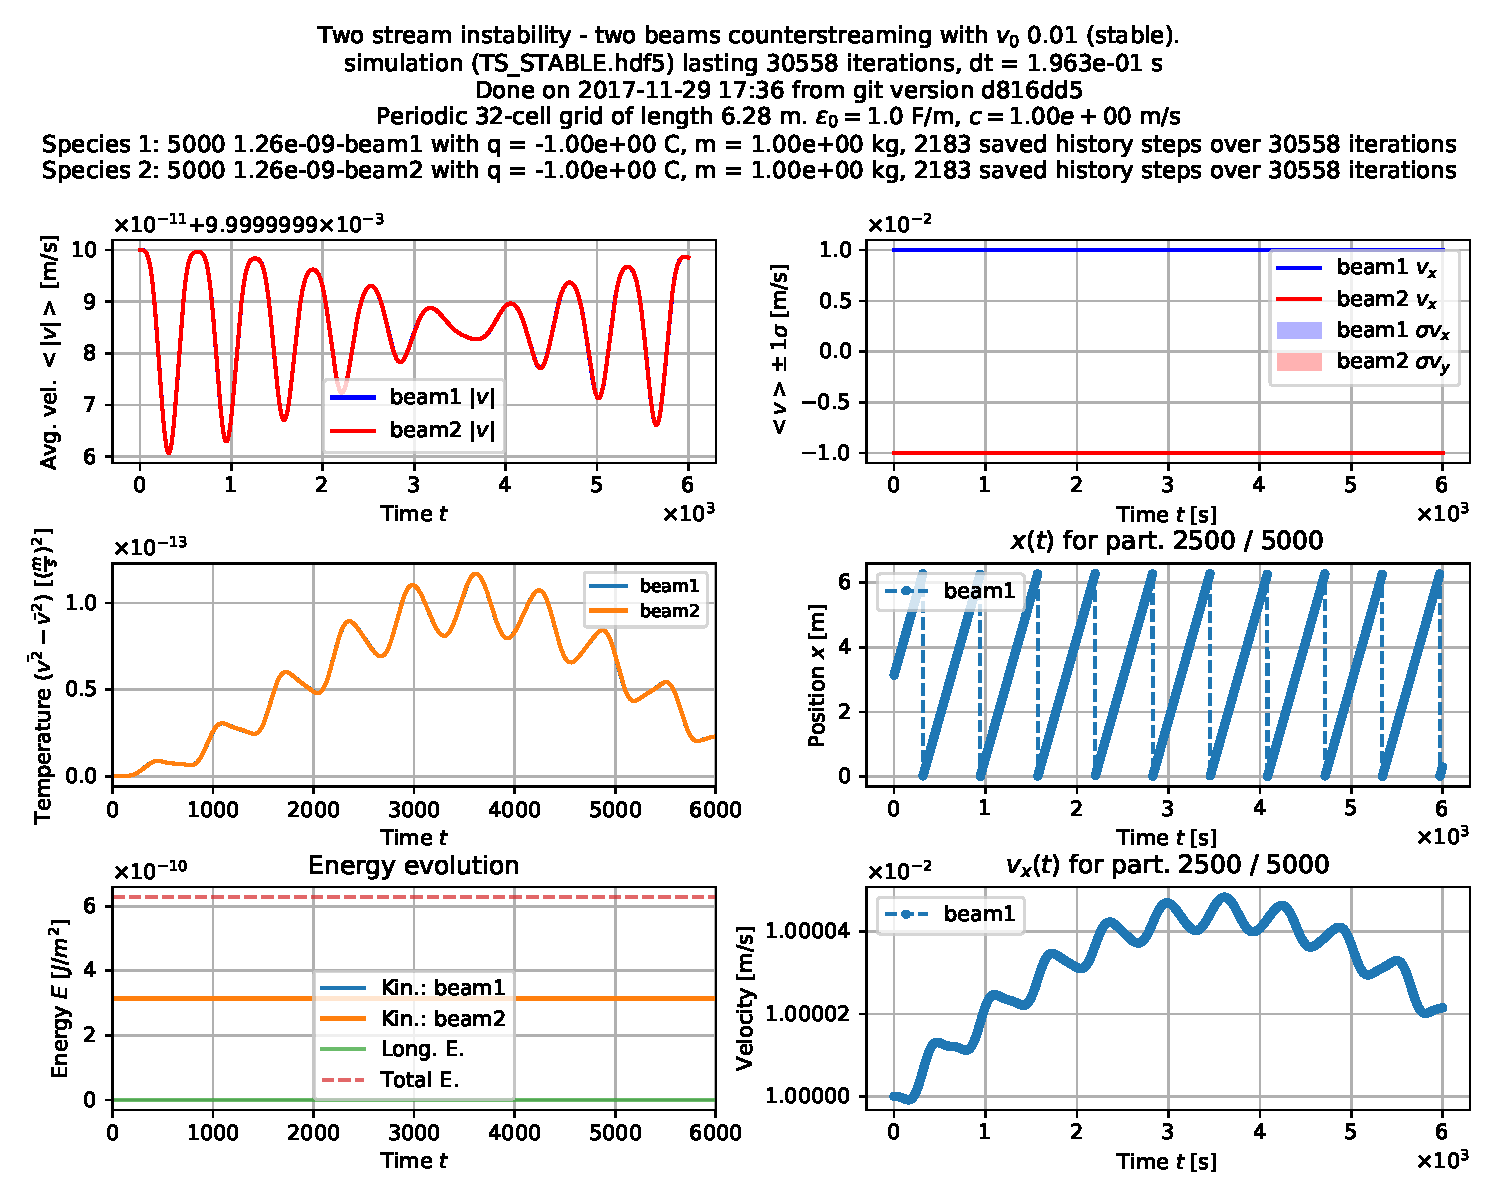
\includegraphics[width=\textwidth]{Images/TS_STABLE}
  \caption{Stabilny reżim dla układu dwóch strumieni. Widoczne są jedynie cykliczny ruch jednostajny w obszarze symulacji i niewielkie zmiany prędkości cząstki.\label{fig:twostream-stable}}
\end{figure}

\begin{figure}[h!]
  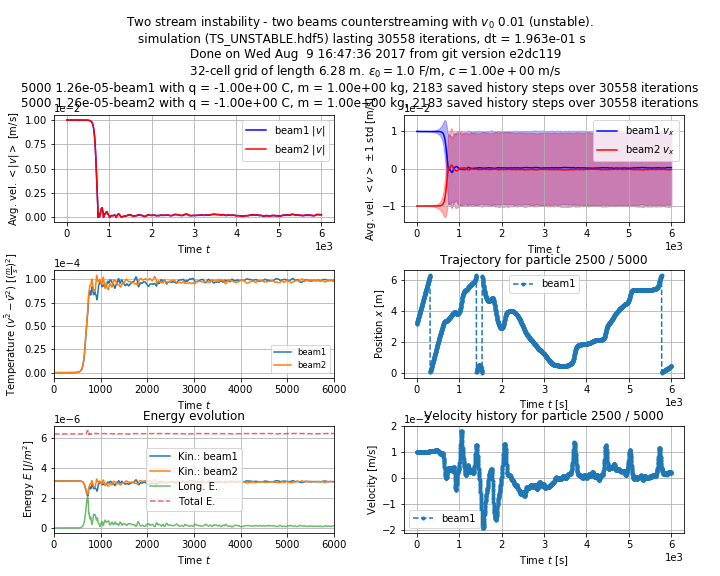
\includegraphics[width=\textwidth]{Images/TS_UNSTABLE}
  \caption{Niestabilny reżim dla układu dwóch strumieni. Trajektoria cząstki staje się chaotyczna.\label{fig:twostream-unstable}}
\end{figure}
% \subsubsection{Oddziaływanie strumienia plazmy z gęstą plazmą tła} % TODO

\subsection{Testowe symulacje elektromagnetyczne --- propagacja fali}
W tym przypadku symulacja nie zawiera plazmy, a badana jest jedynie propagacja fali elektromagnetycznej w obszarze
symulacji dla różnych charakterystyk czasowych. 

Testy jednostkowe obejmują zachowanie energii weryfikowane poprzez zgodność
energii pola elektromagnetycznego w symulacji ze strumieniem Poyntinga generowanym
przez warunek brzegowy. % TODO POYNTING FLUX

% TODO RYSUNEK

\subsection{Symulacja elektromagnetyczna --- oddziaływanie z tarczą wodorową}

Jako warunki początkowe przyjęto plazmę rozbitą na dwie części ---
\emph{preplazmę} o narastającej funkcji rozkładu gęstości oraz plazmę właściwą
o stałej gęstości. Funkcja gęstości jest generowana automatycznie poprzez
metodę opisaną w~\cite{birdsall} i jest normalizowana do danego poziomu
maksymalnej gęstości w obszarze plazmy właściwej przy zadanej liczbie
makrocząstek.

Początkowe prędkości cząstek przyjęto jako zerowe.
% \todo[inline]{wylosowano z relatywistycznego rozkładu Maxwella w kierunkach y, z} % TODO

Za intensywność lasera przyjęto wielkości $10^{21}, 10^{22}, 10^{23} W/m^2$,
zaś za jego długość fali 1.064 $\mu$m (jest to laser Nd:YAG). Przeprowadzono
badania w polaryzacjach liniowej (pole elektryczne w kierunku osi $\hat{y}$ ---
nie zaobserwowano znaczących różnic w symulacji, w której pole elektryczne
skierowano w kierunku osi $\hat{z}$) %TODO CHECK
oraz kołowej wiązki laserowej.

Długość obszaru symulacji to około $10.6 \mu$m, podzielone na 1378 komórek siatki.

\begin{figure}[h!]
  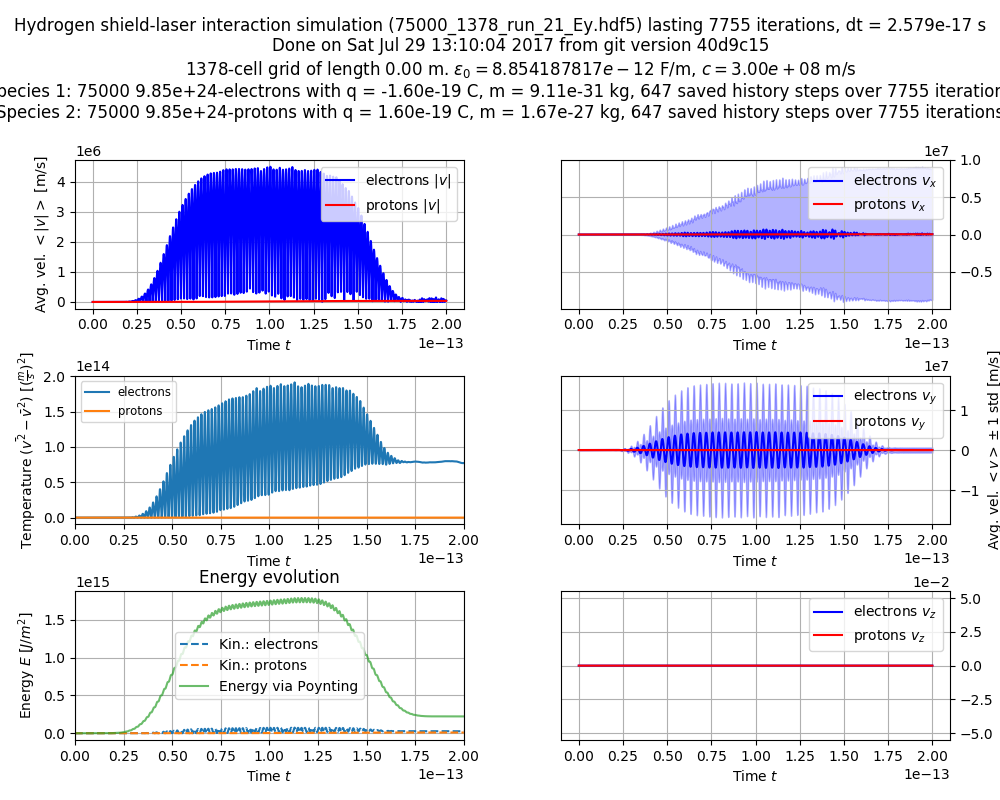
\includegraphics[width=\textwidth]{Images/75000_1378_run_21_Ey}
  \caption{Intensywność wiązki laserowej $10^{21} J/m^2$, polaryzacja liniowa.\label{fig:laser-21-Ey}}
\end{figure}

\begin{figure}[h!]
  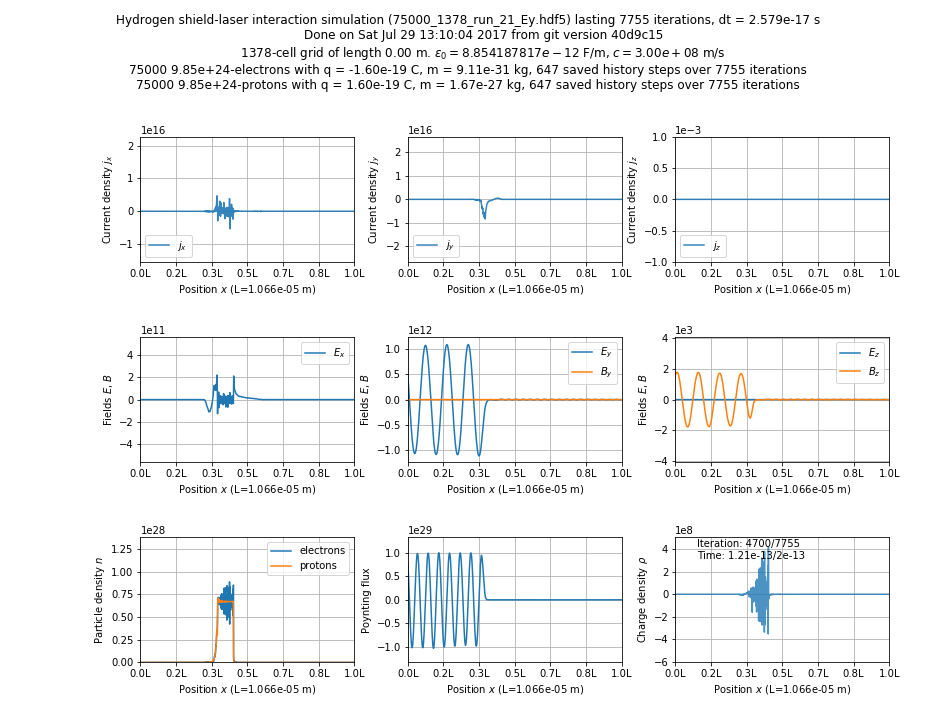
\includegraphics[width=\textwidth]{Images/75000_1378_run_21_Ey_004700}
  \caption{Intensywność wiązki laserowej $10^{21} J/m^2$, polaryzacja liniowa. Rzut na iterację 4700/7755.\label{fig:laser-21-Ey-snapshot}}
\end{figure}

\begin{figure}[h!]
  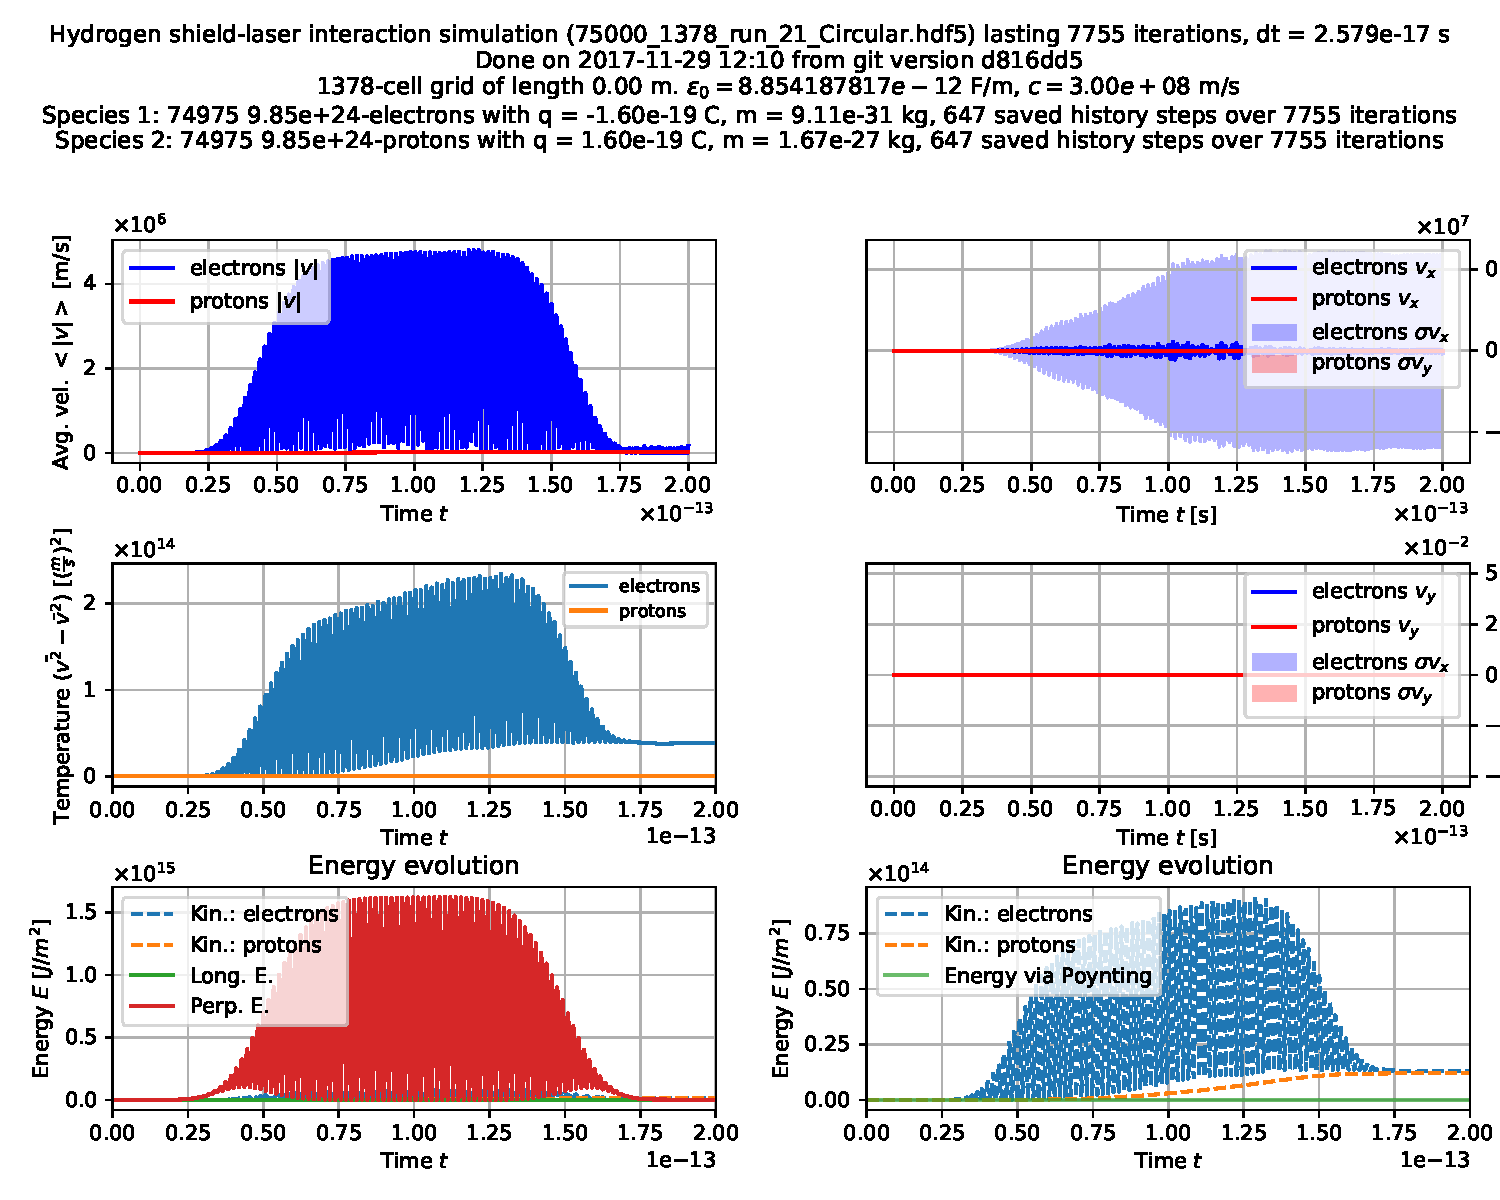
\includegraphics[width=\textwidth]{Images/75000_1378_run_21_Circular}
  \caption{Intensywność wiązki laserowej $10^{21} J/m^2$, polaryzacja kołowa.\label{fig:laser-21-Circular}}
\end{figure}

\begin{figure}[h!]
  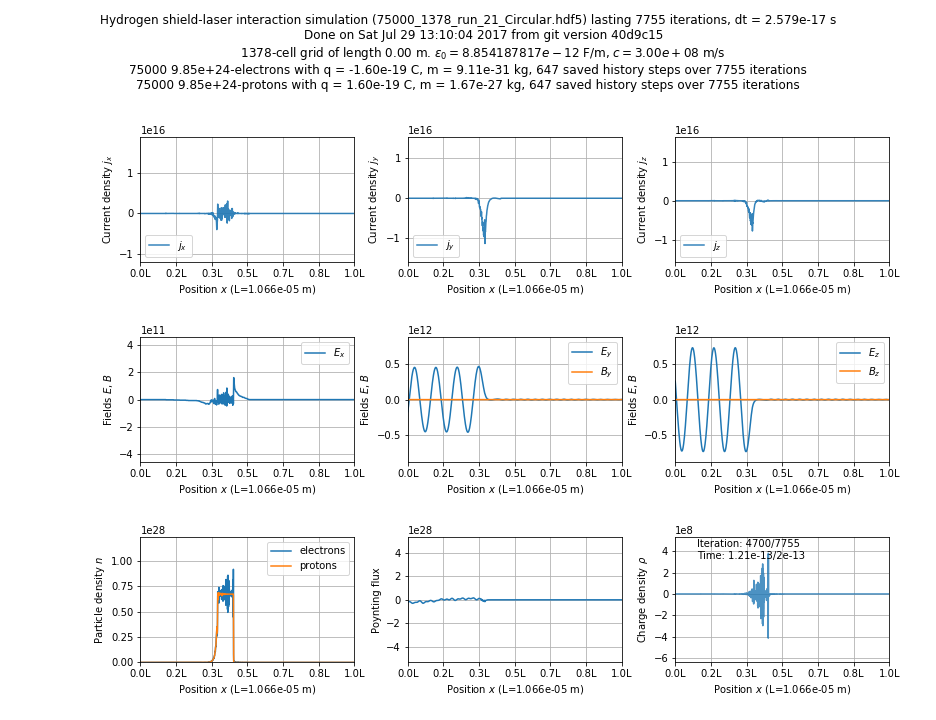
\includegraphics[width=\textwidth]{Images/75000_1378_run_21_Circular_004700}
  \caption{Intensywność wiązki laserowej $10^{21} J/m^2$, polaryzacja kołowa. Rzut na iterację 4700/7755.\label{fig:laser-21-Circular-snapshot}}
\end{figure}

\begin{figure}[h!]
  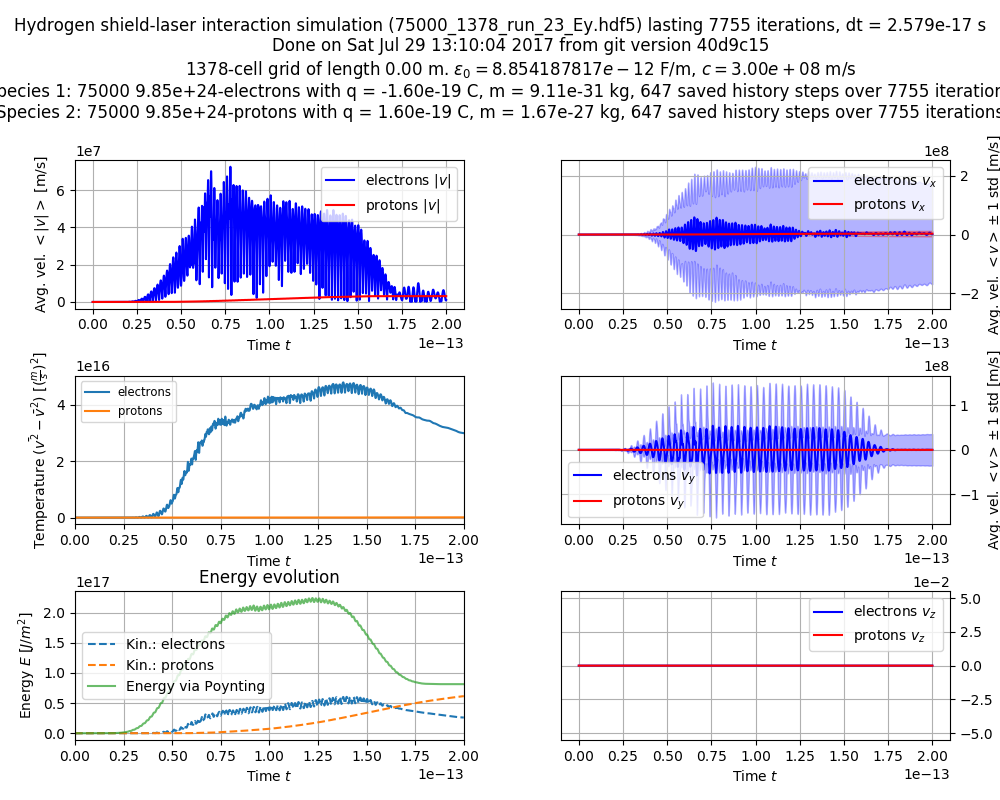
\includegraphics[width=\textwidth]{Images/75000_1378_run_23_Ey}
  \caption{Intensywność wiązki laserowej $10^{23} J/m^2$, polaryzacja liniowa.\label{fig:laser-23-Ey}}
\end{figure}

\begin{figure}[h!]
  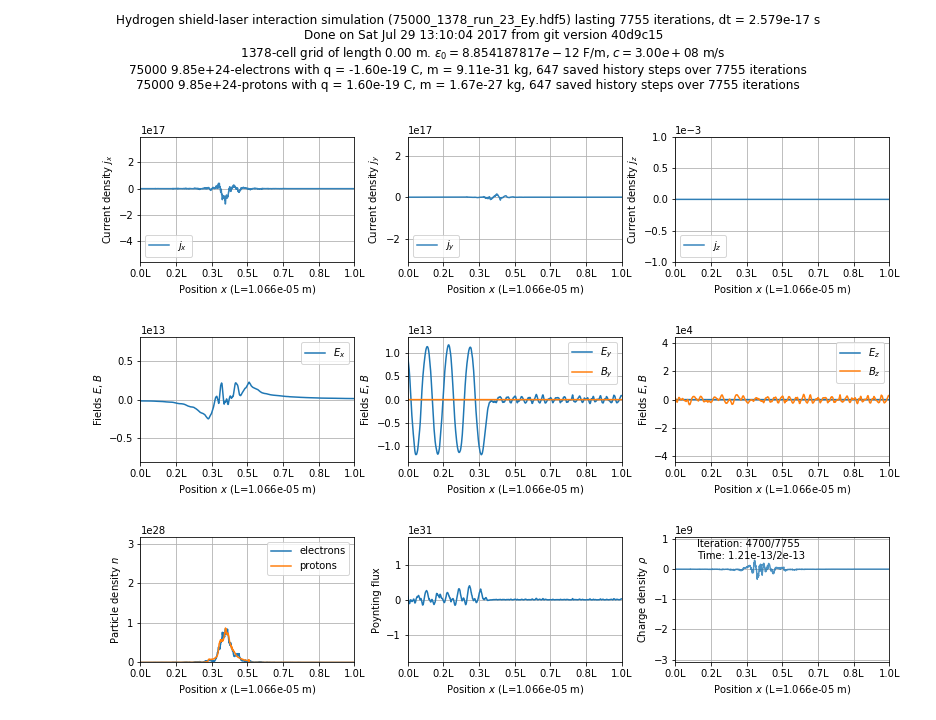
\includegraphics[width=\textwidth]{Images/75000_1378_run_23_Ey_004700}
  \caption{Intensywność wiązki laserowej $10^{23} J/m^2$, polaryzacja liniowa. Rzut na iterację 4700/7755.\label{fig:laser-23-Ey-snapshot}}
\end{figure}


\begin{figure}[h!]
  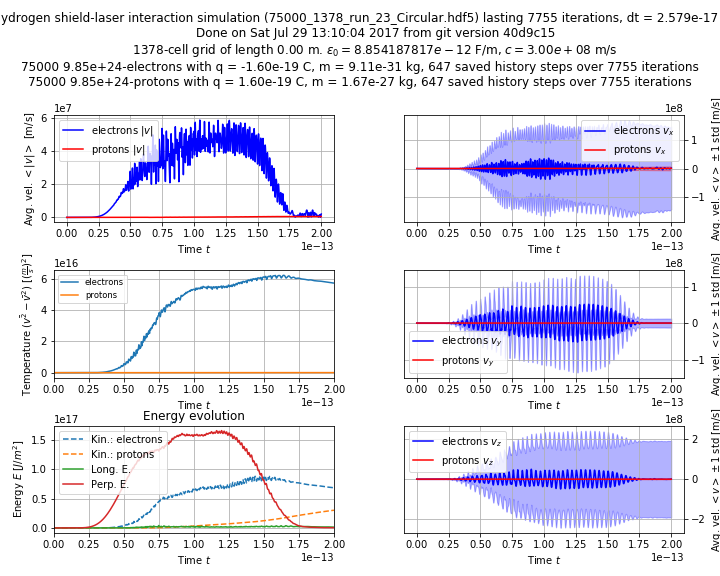
\includegraphics[width=\textwidth]{Images/75000_1378_run_23_Circular}
  \caption{Intensywność wiązki laserowej $10^{23} J/m^2$, polaryzacja kołowa.\label{fig:laser-23-Circular}}
\end{figure}

\begin{figure}[h!]
  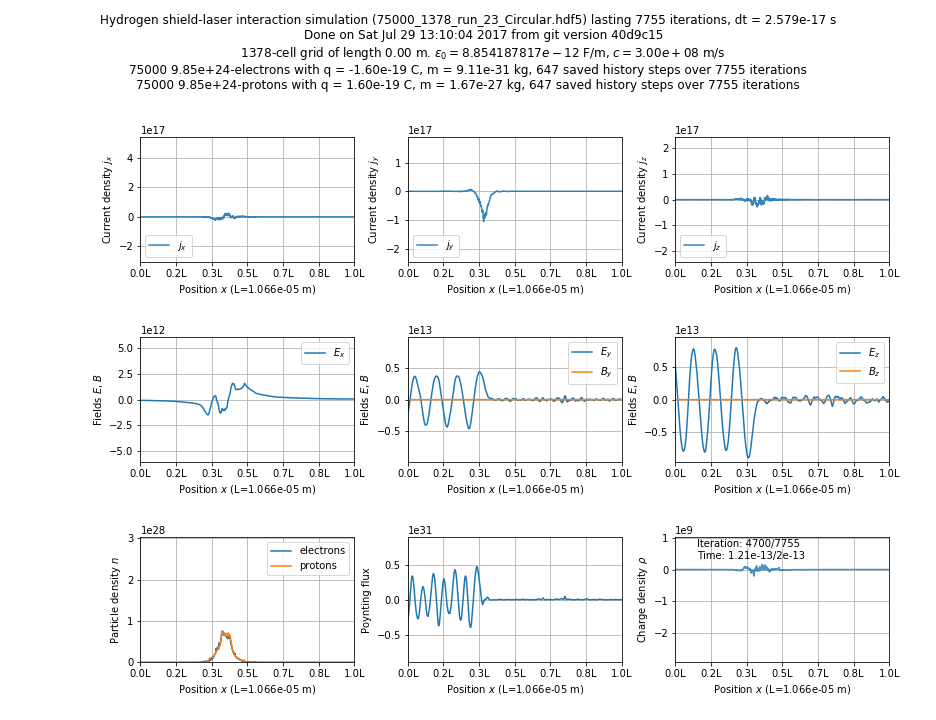
\includegraphics[width=\textwidth]{Images/75000_1378_run_23_Circular_004700}
  \caption{Intensywność wiązki laserowej $10^{23} J/m^2$, polaryzacja kołowa. Rzut na iterację 4700/7755.\label{fig:laser-23-Circular-snapshot}}
\end{figure}




\subsection{Profilowanie}
W celu zmierzenia wydajności kodu zastosowano następujące techniki:
\subsubsection{cProfile}
Uruchamianie kodu w celu zmierzenia wydajności polegało na uruchomieniu skryptu \code{make benchmark}, który:
\begin{enumerate}
\item Czyści zawartość folderu \code{data\_analysis}
\item Uruchamia środowisko Anaconda zawierające bardziej zoptymalizowane od zwyczajnych wersje biblioteki Numpy
\item Uruchamia skrypt \code{fulllaser.py} w trybie \code{cProfile} i zapisuje dane
\end{enumerate}

Następnie zapisane dane są wizualizowane programem \code{snakeviz}.

Za wskaźnik efektów optymalizacji przyjęto całkowity czas trwania symulacji oraz ułamek tego czasu spędzony w funkcji
\code{iteration}.
\subsubsection{line\_profiler}
\subsubsection{IPython timeit}

\subsection{Problemy napotkane w trakcie pisania kodu} % TODO
